%
% Niniejszy plik stanowi przykład formatowania pracy magisterskiej na
% Wydziale MIM UW.  Szkielet użytych poleceń można wykorzystywać do
% woli, np. formatujac wlasna prace.
%
% Zawartosc merytoryczna stanowi oryginalnosiagniecie
% naukowosciowe Marcina Wolinskiego.  Wszelkie prawa zastrzeżone.
%
% Copyright (c) 2001 by Marcin Woliński <M.Wolinski@gust.org.pl>
% Poprawki spowodowane zmianami przepisów - Marcin Szczuka, 1.10.2004
% Poprawki spowodowane zmianami przepisow i ujednolicenie 
% - Seweryn Karłowicz, 05.05.2006
% Dodanie wielu autorów i tłumaczenia na angielski - Kuba Pochrybniak, 29.11.2016

% dodaj opcję [licencjacka] dla pracy licencjackiej
% dodaj opcję [en] dla wersji angielskiej (mogą być obie: [licencjacka,en])
\documentclass[licencjacka]{pracamgr}


% Dane magistranta:
\autor{Michał Izworski}{360968}


% Dane magistrantów:
%\autor{Autor Zerowy}{342007}
%\autori{Autor Pierwszy}{342013}
%\autorii{Drugi Autor-Z-Rzędu}{231023}
%\autoriii{Trzeci z Autorów}{777321}
%\autoriv{Autor nr Cztery}{432145}
%\autorv{Autor nr Pięć}{342011}

\title{AlphaSoccer: gra w ,,Piłkarzyki~na~kartce'' za pomocą głębokich sieci neuronowych}


%\tytulang{An implementation of a difference blabalizer based on the theory of $\sigma$ -- $\rho$ phetors}

%kierunek: 
% - matematyka, informacyka, ...
% - Mathematics, Computer Science, ...
\kierunek{Międzykierunkowe Studia Ekonomiczno-Matematyczne}

% informatyka - nie okreslamy zakresu (opcja zakomentowana)
% matematyka - zakres moze pozostac nieokreslony,
% a jesli ma byc okreslony dla pracy mgr,
% to przyjmuje jedna z wartosci:
% {metod matematycznych w finansach}
% {metod matematycznych w ubezpieczeniach}
% {matematyki stosowanej}
% {nauczania matematyki}
% Dla pracy licencjackiej mamy natomiast
% mozliwosc wpisania takiej wartosci zakresu:
% {Jednoczesnych Studiow Ekonomiczno--Matematycznych}

% \zakres{Tu wpisac, jesli trzeba, jedna z opcji podanych wyzej}

% Praca wykonana pod kierunkiem:
% (podać tytuł/stopień imię i nazwisko opiekuna
% Instytut
% ew. Wydział ew. Uczelnia (jeżeli nie MIM UW))
\opiekun{prof. dr hab. Andrzej Skowron\\
  Wydział Matematyki, Informatyki i Mechaniki\\
  }

% miesiąc i~rok:
\date{Czerwiec 2018}

%Podać dziedzinę wg klasyfikacji Socrates-Erasmus:
\dziedzina{ 
%11.0 Matematyka, Informatyka:\\ 
%11.1 Matematyka\\ 
%11.2 Statystyka\\ 
%11.3 Informatyka\\ 
11.4 Sztuczna inteligencja\\ 
%11.5 Nauki aktuarialne\\
%11.9 Inne nauki matematyczne i informatyczne
}

%Klasyfikacja tematyczna wedlug AMS (matematyka) lub ACM (informatyka)
\klasyfikacja{Computing methodologies\\
	Machine learning\\
 	Learning paradigms\\
	Reinforcement learning\\
	Sequential decision making}

% Słowa kluczowe:
\keywords{machine learning, reinforcement learning, deep learning, actor-critic methods, monte carlo tree search}

% Tu jest dobre miejsce na Twoje własne makra i~środowiska:
\newtheorem{defi}{Definicja}[section]
\usepackage{wrapfig}
\usepackage{graphicx}
\graphicspath{ {img/} }
\usepackage{amsfonts}
\usepackage{amsmath}
\usepackage{algorithm}
\usepackage[noend]{algpseudocode}


\makeatletter
\def\BState{\State\hskip-\ALG@thistlm}
\makeatother

% koniec definicji

\begin{document}

\maketitle

%tu idzie streszczenie na strone poczatkowa
\begin{abstract}
  TO DO
\end{abstract}

\tableofcontents
%\listoffigures
%\listoftables

\chapter{Wprowadzenie}\label{r:intro}

%Sztuczna inteligencja cieszy się ogromnym wzrostem zainteresowania w ostatnim czasie, zarówno wśród społeczności naukowej, jak i w przemyśle. Swoją popularność zawdzięcza temu, iż dzięki niej jesteśmy w stanie poradzić sobie z problemami, których rozwiązania przy użyciu programów komputerowych przynosiły bardzo mierne rezultaty. 
%Na szczególną uwagę zasługuje Uczenie Maszynowe (ang. Machine Learning), które jest obecnie wiodącym nurtem i przyciąga największą uwagę ze względu na najlepsze rezultaty.
%Pozwoliło nam ono na tworzenie programów do rozpoznawania obrazów, tłumaczenia maszynowego czy generowania muzyki. 
%Sztuczna inteligencja okazała się 

%Uczenie Maszynowe cieszy się ogromnym wzrostem zainteresowania w ostatnim czasie, zarówno wśród społeczności naukowej, jak i w przemyśle.
%Pozwoliło nam ono na rozwiązanie problemów, których wcześniejsze próby rozwiązania dawały kiepskie rezultaty, takich jak rozpoznawania obrazów, tłumaczenia maszynowego czy generowania muzyki.
%Jednym z przełomowych wyników sztucznej inteligencji, jakie udało nam się uzyskać

%\section{Intro}

Interakcja z otoczeniem jest prawdopodobnie dla większości z nas naturalnym sposobem uczenia się. 
Dziecko uczące się stawiać pierwsze kroki nie posiada nauczyciela, który dokładnie instruuje je w jaki sposób powinno układać nogi, aby zachować równowagę. 
Zamiast tego, poprzez metodę prób i błędów, stara się ono zrozumieć w jaki sposób zrealizować swój cel i poznaje jakie efekty przynosi wykonywanie przez nie konkretnych ruchów. 
W ten sam sposób uczymy się przez całe życie, jednocześnie poznając otaczający nas świat oraz prawa, które nim rządzą, bez względu na to czy jest to nauka jazdy samochodem czy gry w szachy.

%\section{Intro2}

\section{Piłkarzyki na kartce}

Piłkarzyki na kartce to gra strategiczna, odbywającą się na prostokątnym boisku, rysowanym zazwyczaj na kartce w kratę.
Gracze na przemian wykonują ruchy polegające na przemieszczeniu piłki na sąsiednie pola, aż znajdzie się ona w jednej z bramek lub nie będzie możliwe wykonanie kolejnego ruchu.

\begin{figure}[ht]
  \centering
  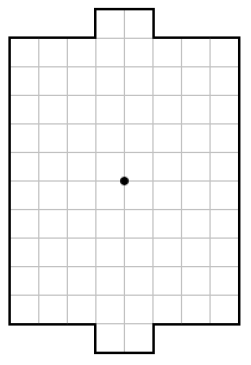
\includegraphics[width=0.2\textwidth]{board}
  \caption{Pusta plansza}
\end{figure}

Najczęściej stosowanym wymiarem planszy jest 8x10 kratek.
Przy krótszych bokach narysowane są dwie bramki o szerokości 2 kratek, w których gracze muszą umieścić piłkę.
Rozgrywka toczy się jedynie na przecięciach linii.
Środek planszy jest punktem startowym gry, do którego gracze dorysowują kolejne linie, oznaczające przemieszczenie piłki na sąsiednie pole. Każdy kolejny ruch zaczyna się w miejscu, w którym skończył się poprzedni, wzdłuż kratki lub po przekątnej. 

Ruchy nie mogą odbywać się po brzegu planszy ani wzdłuż odcinków, po których wcześniej piłka była już prowadzona.
Możliwe jest odbijanie się, które polega na wykonaniu przez gracza dodatkowego ruchu. Następuje ono gdy ruch zostanie zakończony w miejscu, w którym kończy się już linia narysowana przez jednego z graczy lub na brzegu boiska. 

\begin{figure}[ht]
  \centering
  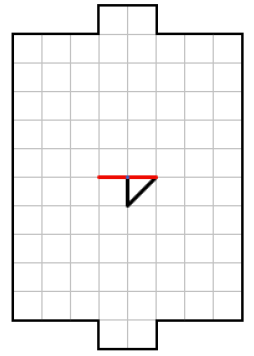
\includegraphics[width=0.2\textwidth]{odbicie}
  \caption{Odbicie (kolor czerwony)}
\end{figure}

Gra kończy się w momencie gdy piłka znajdzie się w jednej z bramek.
Wówczas gracz, do którego należy dana bramka, przegrywa. 
Gracz może również przegrać w wypadku gdy nie jest w stanie wykonać żadnego ruchu.


\begin{figure}[ht]
  \centering
  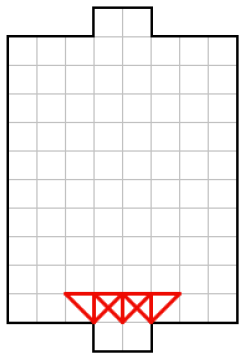
\includegraphics[width=0.2\textwidth]{zablokowanie}
  \caption{Zablokowana bramka}
\end{figure}
 
\section{Cel badawczy} 
 
\section{Podejście} 

\section{Wkład własny}

\section{Zarys pracy}
 
\chapter{Uczenie ze Wzmocnieniem}\label{r:rl}

\section{Wprowadzenie}

Uczenie ze wzmocnieniem (ang. Reinforcement Learning, RL) jest działem uczenia maszynowego, zajmującym się sekwencyjnym podejmowaniem decyzji. Na proces uczenia składa się \emph{agent}, który uczy się podejmować decyzje oraz \emph{środowisko}, które stanowi cały świat zewnętrzy dla agenta. Interakcja między nimi polega na naprzemiennym wykonywaniu akcji przez agenta oraz prezentowaniu nowej sytuacji, w której on się znalazł i nagrody jaką otrzymał przez środowisko. Celem agenta jest maksymalizacja nagród, które otrzymuje.
Podczas procesu uczenia się, nigdy nie wskazujemy agentowi którą akcje powinien on wykonać, co stanowi główną różnice pomiędzy uczeniem ze wzmocnieniem a uczeniem nadzorowanym (ang. Supervised Learning). 

\section{Dyskretny Proces Markowa}

Dyskretny Proces Markowa składa się z:
\begin{itemize}
\item zbioru stanów w których może znaleźć się agent, $ s \in \mathcal{S} $,
\item rozkładu stanu początkowego $\mathcal{D}$ nad zbiorem $\mathcal{S}$,
\item zbioru akcji możliwych do podjęcia przez agenta, $ a \in \mathcal{A} $
\item nagrody otrzymywanej przez agenta za każdym razem, gdy ten wykona jakąś akcje, $ r_t \in \mathbb{R} $
\item prawdopodobieństwa przejścia między stanami
$$ p(s'|s, a) = \mathbb{P}(s_{t+1} = s' \mid s_t = s, a_t = a)$$
\item funkcji nagrody, $ R : S \times S \times A \rightarrow \mathbb{R} $
$$ R(s, a, s') = \mathbb{E}(r_{t+1} \mid s_t = s, a_t = a, s_{t+1} = s') $$
\item współczynnik dyskontującego wartości nagród otrzymywanych w przyszłości $ \gamma \in [0, 1] $
\end{itemize}


\section{Wynik oraz epizody}

Interakcja między agentem a środowiskiem zachodzi w każdym, dyskretnym punkcie czasu $ t = 0, 1, 2, ... $. Znajdując się w punkcie czasu $t$, agent obserwuje stan $ s_t \in \mathcal{S} $, w którym się znajduję, na jego podstawie wykonuje akcję $ a_t \in \mathcal{A}(s) $, gdzie $ \mathcal{A}(s) $ jest zbiorem wszystkich akcji, które można wykonać znajdując się w stanie $s$. W kolejnym kroku dowiaduje się on jaką nagrodę $ r_{t+1} \in \mathbb{R} $ otrzymał i do jakiego stanu $ s_t{t+1} $ się przeniósł. W wyniku otrzymujemy następujący ciąg stanów, akcji oraz nagród, zwany \emph{trajektorią}:

$$ s_0, a_0, r_1, s_1, a_1, r_2, ... $$


\begin{figure}[ht]
  \centering
  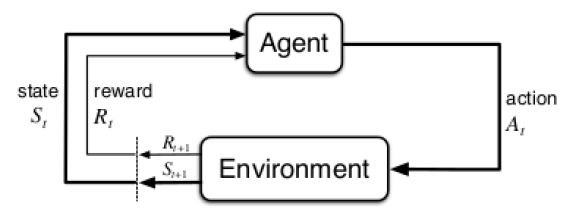
\includegraphics[width=0.5\textwidth]{agent_env_interaction}
  \caption{Interakcja między agentem a środowiskiem jako Dyskretny Proces Markowa}
\end{figure}

Najprostszym typem środowisk są te w których ilość kroków jest z góry ograniczona. Pojedynczy ciąg interakcji nazywamy wówczas \emph{epizodem}, a ostatni stan obserwowany przez agenta -- \emph{stanem terminalnym}. W tym wypadku epizody są od siebie niezależne, mogą się one kończyć w różnych stanach oraz po różnej ilości kroków. 

Celem naszego agenta jest maksymalizacja wartości oczekiwanej sumy nagród, które zdobędzie on w przyszłości. Określmy ją jako \emph{wynik}, $ G_t $, który zdefiniowany jest następująco:

$$ G_t = r_{t+1} + r_{t+2} + r_{t+3} + ... + r_{T-1} = r_{t+1} + G_{t+1} $$

gdzie $T$ jest końcem epizodu, a $t$ indeksem czasu. Sam problem nauczenia naszego agenta w jaki sposób powinien on podejmować decyzje, aby osiągnąć najwyższy wynik, nazywamy \emph{epizodycznym zadaniem}.

Możemy również spotkać się ze środowiskami, z którymi interakcja przebiega nieprzerwanie. Mamy wówczas do czynienia z \emph{ciągłym zadaniem}. Wprowadzamy wówczas koncepcje \emph{dyskontowania} wyniku, który definiujemy następująco:

$$ G_t = r_{t+1} + \gamma r_{t+2} + \gamma^2 r_{t+3} + ... = 
\sum_{k=0}^{\infty} \gamma^k r_{t+k+1} $$

gdzie $ \gamma \in [0, 1) $.


\section{Polityka}

Polityka jest funkcją która każdemu stanowi przyporządkowuje akcję. Może być ona deterministyczna, $ \pi(s) $, bądź też stochastyczna, $ \pi(a \mid s) $, i wówczas stanowić rozkład prawdopodobieństwa wszystkich akcji dla ustalonego stanu. Metody uczenia ze wzmocnieniem określają w jaki sposób polityka jest modyfikowana na podstawie doświadczenia zbieranego przez agenta.

\section{Funkcja Wartości}

Posiadając już politykę naszego agenta, możemy chcieć się dowiedzieć jaką nagrodę uzyska agent, który będzie jej przestrzegał. W tym celu definiujemy \emph{funkcję wartości stanu} (ang. Value Function), którą oznaczamy jako $ v_{\pi}(s) $ dla ustalonej polityki $ \pi $. Definiujemy ją jako:

$$ v_{\pi}(s) = \mathbb{E}_{\pi}[G_t \mid S_t = s] = \mathbb{E}_{\pi} \Bigg[ \sum_{k=0}^{\infty} \gamma^k R_{t+k+1} \bigg| S_t = s \Bigg] $$

gdzie $ \mathbb{E}_{\pi} $ jest wartością oczekiwaną przy założeniu że agent kieruje się polityką $\pi$, z kolei $t$ jest dowolnym punktem w czasie. 

Podobnie definiujemy wartość wybrania akcji $a$, gdy znajdujemy się w stanie $s$ oraz podążamy zgodnie z polityką $\pi$, oznaczaną jako $q_{\pi}(s, a)$. Jest ona wartością oczekiwaną z sytuacji w której rozpoczynamy w stanie $s$, wykonujemy akcję $a$, po czym wszystkie kolejne akcje wykonujemy zgodnie z polityką $\pi$. Funkcję tę nazywamy \emph{funkcją wartości akcji} lub \emph{Q-funkcją}.

$$ q_{\pi}(s, a) = \mathbb{E}_{\pi}[G_t \mid S_t = s, A_t = a] = \mathbb{E}_{\pi} \Bigg[ \sum_{k=0}^{\infty} \gamma^k R_{t+k+1} \bigg| S_t = s, A_t = a \Bigg] $$

\section{Optymalność polityki oraz funkcji wartości}

Podczas rozwiązywania problemu uczenia ze wzmocnieniem staramy się znaleźć politykę, której przestrzeganie przyniesie naszemu agentowi jak największą nagrodę. Będziemy mówić że polityka $\pi$ jest lepsza lub równa polityce $\pi'$, wtedy i tylko wtedy gdy oczekiwana nagroda dla niej jest większa lub równa niż dla $\pi'$ w każdym stanie należącym do przestrzeni stanów. Zawsze istnieje polityka, która jest lepsza lub równa od wszystkich innych i nazywamy ją \emph{optymalną polityką}. Może istnieć wiele różnych od siebie optymalnych polityk, jednak każdą z nich oznaczamy jako $\pi_{\ast}$. Dla wszystkich z nich funkcja wartości stanu jest taka sama i nazywamy ją \emph{optymalną funkcją wartości stanu}. Spełnia ona własność:

$$ v_{\ast}(s) = \max_{\pi} v_{\pi}(s) $$

dla każdego stanu $s \in \mathcal{S}$. Podobnie współdzielą one \emph{optymalną funkcję wartości akcji}, $q_{\ast}$, która spełnia:

$$ q_{\ast}(s, a) = \max_{\pi} q_{\pi}(s, a) $$

dla każdego stanu $s \in \mathcal{S}$ oraz akcji $a \in \mathcal{A}$.

Ponadto optymalną funkcję wartości stanu możemy zdefiniować odwołując się do funkcji wartości akcji w następujący sposób:

$$ v_{\ast}(s) = \max_{a \in \mathcal{A}} q_{\pi_{\ast}}(s) $$

Podstawową własnością, jaką spełniają funkcje wartości, jest \emph{równanie Bellmana}. Dla dowolnej polityki $\pi$ oraz stanu $s$ zachodzi:

\begin{align}
v_{\pi}(s) &= \mathbb{E}_{\pi}[G_t \mid S_t = s]  \nonumber \\
&= \mathbb{E}_{\pi}[r_{t+1} + \gamma G_{t+1} \mid S_t = s] \nonumber \\
&= \sum_a \pi(a \mid s) \sum_s' \sum_r p(s', r \mid s, a) \Big[r + \gamma \mathbb{E}_{\pi}[G_{t+1} \mid S_{t+1} = s' ]\Big] \nonumber \\
&= \sum_a \pi(a \mid s) \sum_{s', r} p(s', r \mid s, a) \Big[r + \gamma v_{\pi}(s') \Big]
\end{align}

Na podstawie własności optymalnych funkcji wartości oraz równania Bellmana możemy wyprowadzić \emph{równania optymalności Bellmana}, bez odwoływania się przy tym do żadnej polityki. Pierwsze z nich odnosi się do funkcji wartości stanu:

\begin{align}
v_{\ast}(s) &= \max_{a \in \mathcal{A}} q_{\pi_{\ast}}(s, a) \nonumber \\
&= \max_a \mathbb{E}_{\pi}[G_t \mid S_t = s, A_t = a]  \nonumber \\
&= \max_a \mathbb{E}_{\pi}[r_{t+1} + \gamma G_{t+1} \mid S_t = s, A_t = a] \nonumber \\
&= \max_a \mathbb{E}[r_{t+1} + \gamma v_{\pi_{\ast}}(S_{t+1}) \mid S_t = s, A_t = a] \nonumber \\
&= \max_a \sum_{s', r} p(s', r \mid s, a) \Big[r + \gamma v_{\ast}(s') \Big]
\end{align}

Natomiast drugie zdefiniowane jest dla funkcji wartości akcji:

\begin{align}
q_{\ast}(s, a) &= \mathbb{E}[r_{t+1} + \gamma \max_{a'} q_{\ast} (S_{t+1}, a') \mid S_t = s, A_t = a] \nonumber \\
&= \sum_{s', r} p(s', r \mid s, a) \Big[r + \gamma \max_{a'} q_{\ast} (s', a') \Big]
\end{align}

\section{Metody uczenia ze wzmocnieniem}

Metody rozwiązywania problemu uczenia ze wzmocnieniem możemy podzielić ze względu na to, czy wykorzystują one model środowiska. Metody \emph{model-based} wymagają od nas \emph{modelu} środowiska, z którego nasz agent będzie korzystał podczas aby przewidzieć w jaki sposób środowisko będzie zachowywało się w odpowiedzi na wykonywane przez niego akcje.
Dzięki temu możliwe jest \emph{planowanie}, które pozwala na przewidywanie zachowania środowiska wiele kroków wprzód. Tego typu problemy możemy spotkać przy okazji nauki naszego agenta w Go, gdzie środowisko imitowane jest przez niego samego, podczas gdy gra on sam ze sobą. 
Drugą klasą algorytmów są metody \emph{model-free}, w których agent posiada jedynie politykę oraz funkcję wartości, a samo zachowanie środowiska jest dla niego nieznane i może on obserwować jedynie bezpośrednie skutki swoich działań. Z takimi problemami spotykamy się np. w przypadku gry naszego agenta na Atari, gdzie nie próbujemy dowiedzieć się jakie prawa rządzą poszczególnymi grami, a zamiast tego po prostu dajemy naszemu agentowi grać.

\subsection{Metody Monte Carlo}

Metody Monte Carlo korzystają z idei \emph{uogólnionej iteracji polityki}, która składa się z dwóch, przeplatających się ze sobą procesów. Pierwszy krok, nazywany \emph{krokiem ewaluacji polityki}, polega na aproksymacji funkcji wartości na podstawie polityki, wykorzystywanej przez agenta. Z kolei w drugim kroku ulepszamy obecną politykę, przy użyciu wcześniej uzyskanej funkcji wartości. Nazywamy go \emph{krokiem ulepszania polityki}.

W przypadku metod Monte Carlo, ewaluacje polityki wykonujemy poprzez próbkowanie kolejnych trajektorii, a następnie wyliczanie średniego wyniku dla każdego ze stanów, bądź każdej pary stan-akcja. Zbierana przez nas historia akcji w postaci trajektorii nazywamy \emph{doświadczeniem} agenta. Najprostszy sposób aktualizacji funkcji wartości może wyglądać następująco:

$$ v(s_t) \leftarrow v(s_t) + \alpha \big[G_t - v(s_t)\big] $$

gdzie $G_t$ oznacza wynik agenta następujący po czasie $t$, a $\alpha$ parametrem wpływającym na szybkość uczenia się.

Ulepszanie polityki następuje poprzez zachłanny wybór najlepszej akcji dla każdego ze stanów, przy pomocy funkcji wartości akcji. Jednak w przypadku takiego doboru polityki, skazujemy się na deterministyczną politykę, która nie jest w stanie odkrywać nowych, potencjalnie lepszych akcji, gdyż cały czas wybierać będzie ona te same akcje. 

Aby utrzymać eksploracje nowych akcji oraz stanów, wprowadzamy pojęcie \emph{$\epsilon$--zachłannej} polityki, która z wysokim prawdopodobieństwem wykonuje akcję, która maksymalizuje wartość funkcji wartości akcji, a od czasu do czasu wykonuje losową akcję. Dzięki temu utrzymujemy stały poziom eksploracji, a przy niewielkich założeniach dla epsilona polityka zbiega do optymalnej.

$$
\pi(a \mid s) =
\begin{cases}
    1 - \epsilon + \epsilon/\lvert \mathcal{A}(s) \rvert & \text{if } a = a^\ast \\
    \epsilon/\lvert \mathcal{A}(s),              & \text{if } a\neq a^\ast
\end{cases}
$$

Metody Monte Carlo cierpią z powodu wysokiej wariancji podczas uczenia, przez co potrzeba bardzo wielu iteracji, aby agent mógł wyuczyć się sensownej polityki. Są one przykładem metod model-free.

\subsection{Temporal-Difference Learning} 

Prawdopodobnie najważniejszą ideą wykorzystywaną  w uczeniu ze wzmocnieniem jest \emph{temporal-difference} (TD) learning. Podobnie do metod Monte Carlo wykorzystuje ono doświadczenie agenta, bez użycia modelu środowiska. Nie jest wymagane jednak oczekiwanie na zakończenie epizodu, aby zaktualizować wartość funkcji wartości, a zamiast tego aktualizacje mogą następować po wykonaniu pojedynczego kroku. Aktualizacja funkcji wartości w przypadku TD learning może wyglądać następująco:

$$ V(S_t) \leftarrow V(S_t) + \alpha \big[R_{t+1} + \gamma V(S_{t+1}) - V(S_t) \big] $$

Sposób tej aktualizacji nazywany jest \emph{TD(0)} lub też \emph{jedno--krokowym} TD, a sam wyraz o który aktualizowana jest wartość:

$$ \delta_t = R_{t+1} + \gamma V(S_{t+1}) - V(S_t) $$

nazywamy \emph{błędem TD}.

\begin{figure}[ht]
  \centering
  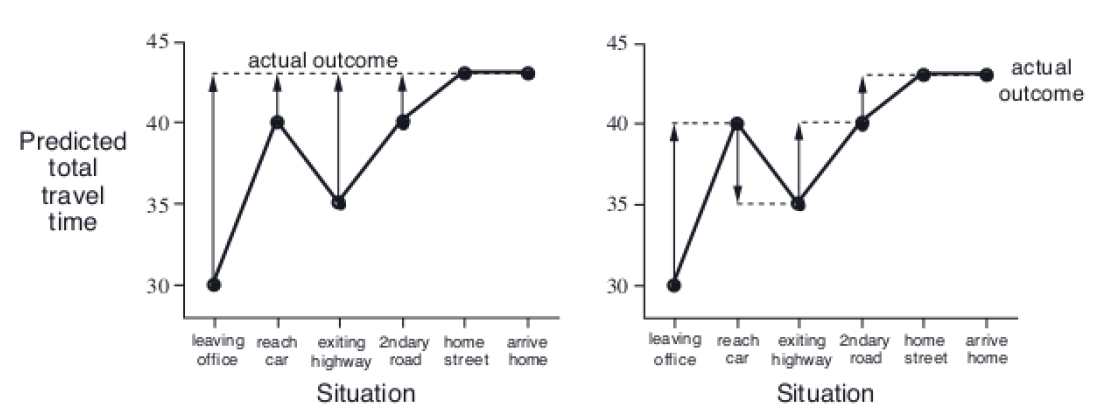
\includegraphics[width=1.0\textwidth]{mc_td}
  \caption{Porównanie aktualizacji funkcji wartości w przypadku metod Monte Carlo (po lewej) oraz metod TD (po prawej)}
\end{figure}

Metody w uczeniu ze wzmocnieniem dzielimy również ze względu na to czy ewaluacja polityki przebiega przy użyciu polityki, która została wykorzystana podczas generowania trajektorii. Metody ewaluujące tę samą politykę nazywamy \emph{on-policy}, natomiast te które działają na różnych politykach nazywamy \emph{off-policy}.

Dwoma podstawowymi algorytmami zaliczającymi się do TD learning jest \emph{SARSA (State-Action-Reward-State-Action} oraz \emph{Q-Learning}.

SARSA jest przykładem metody on-policy, która wykorzystuje funkcję wartości akcji, zamiast funkcji wartości stanu. W przypadku tej metody aktualizacja funkcji wartości akcji jest następująca:

$$ Q(S_t, A_t) \leftarrow Q(S_t, A_t) + \alpha \big[R_{t+1} + \gamma Q(S_{t+1}, A_{t+1}) - Q(S_t, A_t) \big] $$

Aktualizacja ta zachodzi dla każdego nieterminalnego stanu $S_t$, a w przypadku gdy $S_{t+1}$ jest terminalny, to $ Q(S_{t+1}, A_{t+1}) $ definiujemy jako zero. Cały proces zależny jest od piątki $ (S_t, A_t, R_{t+1}, S_{t+1}, A_{t+1}) $, skąd pochodzi nazwa algorytmu \emph{SARSA}.

Q-Learning natomiast jest przykładem metody off-policy, w której aktualizacja Q-funkcji przebiega następująco:

$$ Q(S_t, A_t) \leftarrow Q(S_t, A_t) + \alpha \big[R_{t+1} + \gamma \max_a Q(S_{t+1}, a) - Q(S_t, A_t) \big] $$

W ten sposób uczona się przez nas funkcja $Q$ bezpośrednio aproksymuje $Q_\ast$, niezależnie od tego jaka polityka jest przez nas wykorzystywana do wybierania kolejnych akcji.

\subsection{Rollout Algorithms}

Metody wykorzystujące model do podejmowania decyzji, nazywane metodami \emph{model-based}, opierają się na planowaniu kolejnych ruchów, które w przyszłości podejmie nasz agent. Główną metodą planowania jest \emph{planowanie w momencie podjęcia decyzji}, które skupia się na podejmowaniu decyzji po znalezieniu się w konkretnym stanie $S_t$, a więc wyborze akcji $A_t$. Najważniejszy dla nas wówczas jest stan, w którym się znaleźliśmy, mniej natomiast te odległe bądź już odwiedzone, do których już nigdy nie powrócimy. Niezwykle użyteczne okazują się one w przypadku gdy na podjęcie decyzji możemy poświęcić trochę czasu, jak np. w przypadku szachów czy Go, mniej przydatne będzie ono jeśli nasz program będzie musiał bardzo szybko podejmować decyzje. 

Algorytmy typu rollout są algorytmami planowania w momencie podjęcia decyzji  i bazują na bardzo podobnej zasadzie co metody Monte Carlo. Przybliżają one funkcję wartości akcji dla stanu, w którym się znajdują, za pomocą symulowania kolejnych trajektorii, podobnie jak w przypadku ewaluacji polityki w Monte Carlo. Ich celem jednak nie jest znalezienie optymalnej polityki $\pi_\ast$ czy też funkcji $q_\ast$, a zamiast tego służą nam do stworzenia \emph{rollout polityki} za każdym razem gdy znajdziemy się w jakimś stanie. Okazuje się że polityki otrzymane w ten sposób radzą sobie nadzwyczaj dobrze.

\subsection{Monte Carlo Tree Search}

Przeszukiwanie drzew metodą Monte Carlo, czyli \emph{Monte Carlo Tree Search (MCTS)} jest dość nowym podejściem w uczeniu ze wzmocnieniem, wykorzystanym między innymi w takich programach jak AlphaGo. 

MCTS jako algorytm rollout symuluje kolejne trajektorie rozpoczynające się w obecnym stanie, a kończące na stanie terminalnym. Rozszerza on ten pomysł poprzez przechowywanie i aktualizację funkcji wartości akcji dla kolejnych ruchów, zamiast jak to było w poprzednim przypadku, tylko dla stanu w którym się on znajduje. Tworzone jest wówczas drzewo, ukorzenione w obecnym stanie, które wraz z kolejnymi symulacjami się rozszerza i dokładniej aproksymuje Q funkcję. Dla stanów obecnych w drzewie, decyzję podejmujemy na podstawie funkcji wartości zawartej w węzłach drzewa, a politykę wytworzoną w ten sposób nazywamy \emph{polityką drzewa}. Gdy podczas symulowania trajektorii dochodzimy do liścia w naszym drzewie, to dalsza symulacja wykonywana jest na podstawie rollout polityki. Eksporacja zapewniona jest na poziomie polityki drzewa, na przykład za pomocą zastosowania polityki $\epsilon$-zachłannej.

Pojedyncza iteracja MCTS dzieli się na cztery kroki:

\begin{enumerate}
\item \textbf{Wybór.} Wybierane są kolejne stany należące do drzewa na podstawie polityki utworzonej z wartości funkcji akcji, która zdefiniowana jest przez krawędzie grafu. Przejście przez drzewo rozpoczyna się w korzeniu, a kończy w liściu drzewa.
\item \textbf{Rozwinięcie.} Drzewo jest rozszerzane w liściu, który został osiągnięty w poprzednim kroku, poprzez dodanie nowych węzłów jako dzieci dla tego liścia. Nowe węzły reprezentują stany, które wcześniej nie były obecne w drzewie.
\item \textbf{Symulacja.} Zaczynając w węźle wybranym w pierwszym punkcie, rozpoczynana jest symulacja na podstawie polityki rollout. W wyniku otrzymujemy trajektorię, której pierwsze ruchy zostały wybrane za pomocą polityki drzewa, a pozostałe -- polityki rollout.
\item \textbf{Propagacja wsteczna.} Wynik agenta jest propagowany wstecz do aktualizacji istniejących węzłów, bądź utworzenia nowych. Proces ten dotyczy jedynie stanów, które znajdują się w drzewie.
\end{enumerate}


\begin{figure}[ht!]
  \centering
  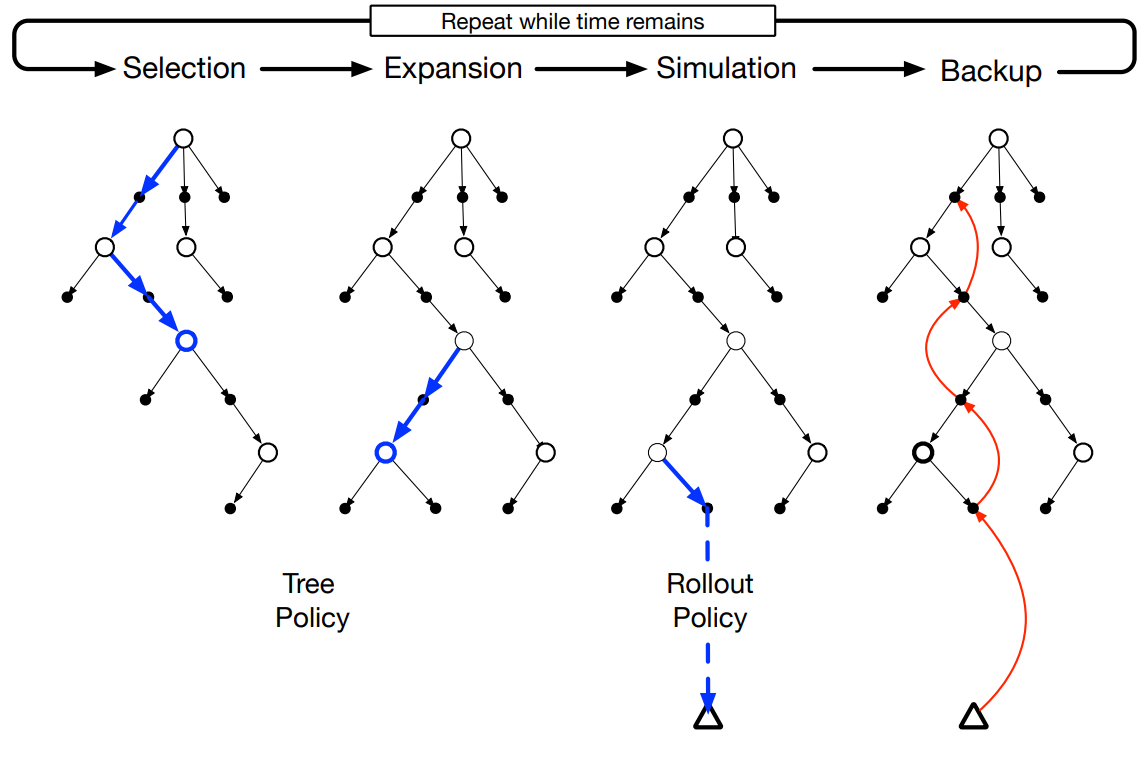
\includegraphics[width=0.85\textwidth]{mcts}
  \caption{Kolejne kroki podczas rozwijania drzewa w MCTS}
\end{figure}


\section{Podsumowanie}

W tym rozdziale zaprezentowane zostały podstawowe podejścia oraz koncepcje stosowane w uczeniu ze wzmocnieniem. Podczas tworzenia programów rozwiązujących gry strategiczne na planszy, jakimi są piłkarzyki na kartce czy Go, będziemy ze sobą łączyć te techniki, wzbogacając je dodatkowo o sieci neuronowe. W kolejnym rozdziale bliżej przyjrzymy się sieciom neuronowym, aby zrozumieć w jaki sposób one działają i jak możemy zastosować je do rozwiązania naszego problemu.

\chapter{Głębokie Sieci Neuronowe}

Ostatnio bardzo często mamy okazję słyszeć o Sztucznych Sieciach Neuronowych. Ponownie stały się one popularne wśród społeczności sztucznej inteligencji i obecnie osiągają najlepsze wyniki w bardzo wielu dziedzinach. Pozwalają nam one nam na tworzenie autonomicznych pojazdów, rozpoznawać obrazy lepiej od ludzi czy pokonać mistrza świata w Go. 

Głębokie Sieci Neuronowe mają zdolność do tworzenia aproksymacji nieliniowych funkcji na podstawie danych. Ponadto, w porównaniu do innych modeli uczenia maszynowego, nie wymagają one ręcznego tworzenia istotnych cech na podstawie danych, a zamiast tego same tworzą własną reprezentacje. Dzięki temu ograniczają one wymaganą interakcje z modelem, przy jednoczesnej poprawie jakości uzyskiwanych cech.

\section{Sieci jednokierunkowe}

Głębokie sieci jednokierunkowe (ang. Deep Feedforward Networks), zwane również wielowarstwowym perceptronem (ang. Multilayer Perceptron), są podstawowym modelem głebokiego uczenia. Ich zadaniem jest przybliżanie funkcji $ y = f^{\ast}(x) $, która dla danych wejściowych $x$ przyporządkowuje konkretną decyzję $y$ np. kategorię. Sieć jest wówczas funkcją $ y = f(x; \theta) $ parametryzowaną przez wektor $\theta$, który uczy się na podstawie danych.

Sieci neuronowe nazywane są sieciami, gdyż są one złożeniem wielu funkcji ze sobą, przez co informacje przepływają kolejno przez wszystkie z nich. Możemy je reprezentować jako acykliczny graf, który definiuje kolejne kroki wykonywanych obliczeń. Przykładowo możemy złożyć ze sobą dwie funkcje $ f(x) = f^{(2)}(f^{(1)}(x)) $, otrzymując sieć w której $f^{(1)} $ jest pierwszą warstwą sieci, a $ f^{(2)} $ -- drugą. Ilość składanych ze sobą sieci nazywamy \emph{głębokością} sieci, ostatnią warstwę -- \emph{warstwą wyjściową}, a pozostałe warstwy -- \emph{ukrytymi warstwami}. 

Sieci jednokierunkowe zawdzięczają swoją nazwę temu, iż przepływ informacji w nich występuje jedynie w jednym kierunku, a więc każda z warstw jest zależna jedynie od poprzednich. Nie występuje w żadne nich sprzężenie zwrotne, które jest charakterystyczne dla rekurencyjnych sieci neuronowych.

Sztuczne sieci neuronowe swoją budową bazują na prawdziwych sieci neuronowych, które występują w mózgu, przez co nawiązują w nich w swojej nazwie. Warstwy sieci scharakteryzowane są przez \emph{szerokość}, która mówi o rozmiarze wektora produkowanego przez odpowiadającą jej funkcję. Każdy element wektora może pełnić wówczas funkcję analogiczną do neurona, który zbiera wszystkie informacje z poprzedniego wektora i tworzy na ich podstawie pewną wartość. Wszystkie neurony w warstwie działają niezależnie od siebie. Pomimo jednak iż głębokie uczenie posiadają swoje korzenie w neuronaukach, to obecnie funkcje są dobierane przez inżynierów na podstawie ich własności matematycznych, a ich głównym celem nie jest już naśladowanie działania mózgu.

\section{Funkcje aktywacji}

\section{Funkcja kosztu}

\section{Algorytm propagacji wstecznej}

\section{Regularyzacja}

\section{Normalizacja batchów}

\section{Konwolucyjne Sieci Neuronowe}

\section{Głębokie Rezydualne Uczenie}

\section{Podsumowanie}

\chapter{Głębokie Uczenie ze Wzmocnieniem}

\section{Wprowadzenie}

\section{Deep Q-Learning}

\section{Policy Gradient}

\section{Actor Critic-Methods}

\section{Podsumowanie}

\chapter{Gra w piłkarzyki na kartce}

\section{Wprowadzenie}

\section{Metoda uczenia poprzez grę z samym sobą}

\subsection{Rozgrywanie gier}

\subsection{Trenowanie na zebranym doświadczeniu}

\subsection{Ewaluacja wyuczonej polityki}

\section{Algorytm przeszukujący drzewo gry}

\subsection{Wybór ścieżki w drzewie}

\subsection{Rozwinięcie i ewaluacja nowego węzła}

\subsection{Propagacja wsteczna}

\subsection{Wybór akcji}

\section{Architektura sieci}

\section{Pierwsze testy na zmniejszonej planszy}

\section{Wyniki dla gry standardowych rozmiarów}

\section{Podsumowanie}

\chapter{Wnioski}

\begin{thebibliography}{99}

\end{thebibliography}

\end{document}


%%% Local Variables:
%%% mode: latex
%%% TeX-master: t
%%% coding: latin-2
%%% End:
